% Consistent but Blind? -- A0 landscape poster. Compile from this folder: `tectonic poster.tex` (or latexmk -pdf).
% Figures are the vector PDFs written by `medvlm posthoc`, `medvlm contrast --analyze` and `medvlm replication`.
\documentclass[25pt, a0paper, landscape, margin=0mm, innermargin=18mm, blockverticalspace=9mm, colspace=16mm,
  subcolspace=8mm]{tikzposter}

\usepackage[T1]{fontenc}
\usepackage[scaled=0.95]{helvet}
\renewcommand{\familydefault}{\sfdefault}
\usepackage{graphicx}
\usepackage{booktabs}
\usepackage{array}
\usepackage{qrcode}
\usepackage{enumitem}
\usepackage{textcomp}
\newcommand{\mn}{\textminus}
\setlist{leftmargin=1.1em, itemsep=0.25em, topsep=0.3em}

% Palette shared with the paper's figures
\definecolor{ink}{HTML}{0B0B0B}
\definecolor{ink2}{HTML}{52514E}
\definecolor{rule}{HTML}{D9DCE1}
\definecolor{med}{HTML}{2A78D6}     % medical model (blue in every figure)
\definecolor{gen}{HTML}{EB6834}     % general base (orange)
\definecolor{dang}{HTML}{E34948}    % the Dangerous quadrant
\definecolor{paper}{HTML}{FCFCFB}
\definecolor{tint}{HTML}{EEF3FB}

\definecolorstyle{cbb}{
  \colorlet{colorOne}{ink}\colorlet{colorTwo}{med}\colorlet{colorThree}{paper}
}{
  \colorlet{backgroundcolor}{paper}\colorlet{framecolor}{paper}
  \colorlet{titlefgcolor}{ink}\colorlet{titlebgcolor}{paper}
  \colorlet{blocktitlefgcolor}{ink}\colorlet{blocktitlebgcolor}{paper}
  \colorlet{blockbodyfgcolor}{ink}\colorlet{blockbodybgcolor}{paper}
  \colorlet{innerblocktitlefgcolor}{ink}\colorlet{innerblocktitlebgcolor}{tint}
  \colorlet{innerblockbodyfgcolor}{ink}\colorlet{innerblockbodybgcolor}{tint}
  \colorlet{notefgcolor}{ink}\colorlet{notebgcolor}{tint}\colorlet{noteframecolor}{tint}
}
\usecolorstyle{cbb}

% Blocks: a bold title over a thin blue rule, no boxes
\defineblockstyle{cbb}{
  titlewidthscale=1, bodywidthscale=1, titlecenter=false, titleoffsetx=0pt, titleoffsety=0pt,
  bodyoffsetx=0pt, bodyoffsety=0pt, bodyverticalshift=0pt, roundedcorners=0, linewidth=0pt,
  titleinnersep=6mm, bodyinnersep=6mm
}{
  \draw[draw=none, fill=blockbodybgcolor] (blockbody.south west) rectangle (blockbody.north east);
  \ifBlockHasTitle
    \draw[draw=none, fill=blocktitlebgcolor] (blocktitle.south west) rectangle (blocktitle.north east);
    \draw[color=med, line width=3mm] (blocktitle.south west) -- (blocktitle.south east);
  \fi
}
\useblockstyle{cbb}
\usebackgroundstyle{Empty}

\definetitlestyle{cbb}{
  width=\paperwidth, roundedcorners=0, linewidth=0pt, innersep=14mm, titletotopverticalspace=0mm,
  titlegraphictotitledistance=10pt
}{
  \draw[draw=none, fill=titlebgcolor] (\titleposleft, \titleposbottom) rectangle (\titleposright, \titlepostop);
  \draw[color=rule, line width=2mm] (\titleposleft, \titleposbottom) -- (\titleposright, \titleposbottom);
}
\usetitlestyle{cbb}

\settitle{%
  \begin{minipage}[c]{0.80\linewidth}\raggedright
    {\color{ink}\fontsize{118}{128}\selectfont\bfseries Consistent but Blind?\par}
    \vspace{6mm}
    {\color{ink}\fontsize{66}{78}\selectfont Image removal does not measure image reliance\\[2mm]
     in medical vision-language models\par}
    \vspace{12mm}
    {\color{ink2}\fontsize{38}{46}\selectfont \textbf{Tri Thai Huu} \;\textperiodcentered\; VinUniversity, Hanoi, Vietnam
      \;\textperiodcentered\; thaitri2005@gmail.com\par}
  \end{minipage}\hfill
  \begin{minipage}[c]{0.16\linewidth}\centering
    \qrcode[height=15cm]{https://github.com/thaitri2005/Medvlm-Image-Reliance}\\[4mm]
    {\color{ink2}\fontsize{26}{30}\selectfont Paper, code, data and\\every number}
  \end{minipage}%
}

\newcommand{\bignum}[1]{{\fontsize{64}{68}\selectfont\bfseries #1}}
\newcommand{\med}[1]{\textcolor{med}{\textbf{#1}}}
\newcommand{\gen}[1]{\textcolor{gen}{\textbf{#1}}}
\newcommand{\dng}{\textcolor{dang}{\textsc{Dangerous}}}
\newcommand{\muted}[1]{\textcolor{ink2}{#1}}

\tikzposterlatexaffectionproofoff

\begin{document}
\maketitle

\begin{columns}
% ------------------------------------------------------------------ column 1
\column{0.285}

\block{The question}{
Medical VQA benchmarks score whether an answer is right, not whether the model \emph{looked}. The
\emph{consistent-but-dangerous} taxonomy (Sadanandan \& Behzadan, 2026) checks both, per answer:

\vspace{6mm}
\begin{center}\renewcommand{\arraystretch}{1.35}
\begin{tabular}{@{}l>{\centering\arraybackslash}p{9.2cm}>{\centering\arraybackslash}p{9.2cm}@{}}
 & \textbf{changes} without the image & \textbf{unchanged} without the image\\
\midrule
\textbf{stable} under paraphrase & \textsc{Ideal} & \dng\\
\textbf{flips} under paraphrase & \textsc{Fragile} & \textsc{Worst}\\
\end{tabular}
\end{center}
\vspace{6mm}

Its reliance axis is \textbf{image removal}. A taxonomy like this invites comparisons: is the medical model more
\dng{} than the general one?

\vspace{4mm}
\innerblock{}{\large We ask: does image removal rank models the way probes that \textbf{keep an image in the
input} do?}
}

\block{Setup}{
\textbf{Three pairs}, each a medical model and the general model it shares an architecture with:
\begin{itemize}
\item \med{MedGemma-4B} and \med{MedGemma-1.5-4B} vs.\ \gen{Gemma-3-4B}
\item \med{MedVLThinker-3B} (RL on PMC-VQA) vs.\ its base \gen{Qwen2.5-VL-3B}
\end{itemize}
\textbf{Data}: SLAKE (CT, MRI, X-ray), VQA-RAD (radiology), PathVQA (pathology): 3,365 questions on 907
images; 1,206 yes/no test questions are the primary set.

\vspace{4mm}
\renewcommand{\arraystretch}{1.25}
\begin{tabular}{@{}p{9.5cm}p{17.5cm}@{}}
\toprule
\textbf{Probe} & \textbf{What changes}\\
\midrule
Image removed & image tokens omitted (the taxonomy's probe)\\
Wrong image & another image, same dataset and modality\\
Black image & a black image in the image slot\\
Opposite-answer image & another image on which the \emph{same question} has the opposite answer\\
``Unknown'' allowed & image removed, the model may decline\\
\bottomrule
\end{tabular}

\vspace{5mm}
bf16, greedy, identical prompts; about 120,000 model calls on one 16\,GB GPU. CIs: 95\%, cluster bootstrap by
image. \textbf{Pre-registered}: endpoints frozen before the main run; every later probe and model pair registered
(a dated git tag) before it was run.
}

% ------------------------------------------------------------------ column 2
\column{0.43}

\block{Finding 1. Image removal agrees with no in-format probe}{
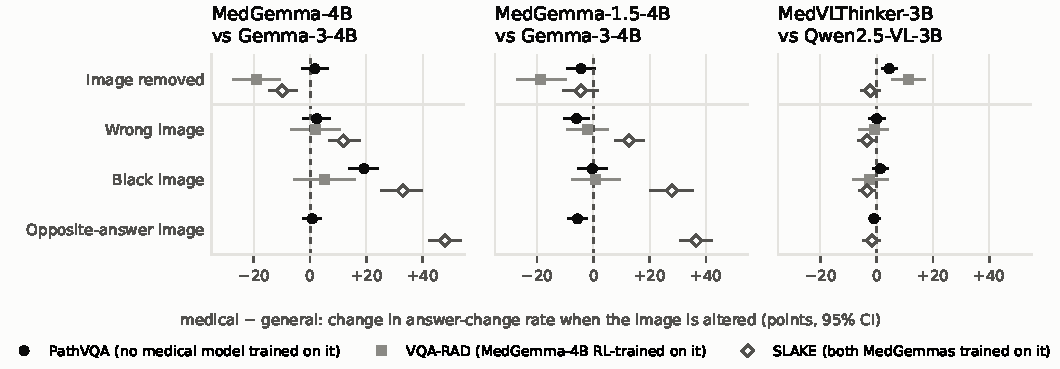
\includegraphics[width=\linewidth]{../figures/fig10_by_dataset.pdf}

\vspace{2mm}
\muted{Medical \mn{} general difference in how often a yes/no answer changes when the image is altered. A model
that uses the image should change its answer when the image changes.}

\vspace{8mm}
\begin{tikzfigure}
\begin{tabular}{@{}c@{\hspace{3cm}}c@{\hspace{3cm}}c@{}}
\bignum{5 of 9} & \bignum{0 of 5} & \bignum{+13.7}\\[3mm]
\begin{minipage}[t]{0.27\linewidth}\centering pair $\times$ dataset cells where image removal separates the
models\end{minipage} &
\begin{minipage}[t]{0.27\linewidth}\centering of those cells where any in-format probe agrees\end{minipage} &
\begin{minipage}[t]{0.27\linewidth}\centering points more \dng{} for MedGemma-4B under image removal\end{minipage}\\
\end{tabular}
\end{tikzfigure}
}

\block{What image removal picks up instead}{
\begin{minipage}[t]{0.56\linewidth}\vspace{0pt}
\textbf{Refusal.} Told to answer yes or no about an image it was not given, \gen{Gemma-3} would rather ask for
it on \textbf{354 of 1,206} questions; \med{MedGemma-4B} on 219, \med{MedGemma-1.5} on 8, the Qwen pair never.
The forced answers there are unrelated to the answers with the image ($\kappa \approx 0$), so about half count as
``image-reliant''. The largest image-removal gaps sit where refusal differs most (VQA-RAD).

\vspace{5mm}
\textbf{Priors that match the image.} A model whose blind guess matches what the image shows gives the same
answer with and without it, and image removal calls that blind. MedGemma-4B's extra \dng{} answers are
\textbf{all correct}: +14.1 correct, \mn0.4 wrong.
\end{minipage}\hfill
\begin{minipage}[t]{0.40\linewidth}\vspace{0pt}
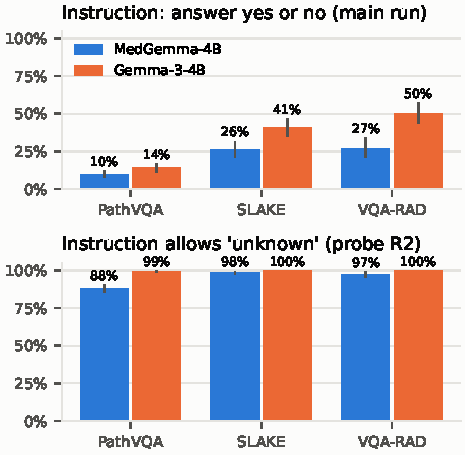
\includegraphics[width=\linewidth]{../figures/fig4_abstention.pdf}

\muted{Share of yes/no questions the model declines without the image. Allowed to say ``unknown'' (bottom),
both decline on $\ge$93\%.}
\end{minipage}
}

% ------------------------------------------------------------------ column 3
\column{0.285}

\block{Finding 2. The in-format advantage stays in the training data}{
The same probe inside and outside the medical models' training data:

\vspace{4mm}
\begin{center}\renewcommand{\arraystretch}{1.3}
\begin{tabular}{@{}lrr@{}}
\toprule
Follows the opposite-answer image, & \textbf{SLAKE} & \textbf{PathVQA}\\
medical \mn{} general (points) & (trained on) & (held out)\\
\midrule
\med{MedGemma-4B} \mn{} \gen{Gemma-3} & +48.0 & +0.8 \muted{[\mn2.7, 4.2]}\\
\med{MedGemma-1.5} \mn{} \gen{Gemma-3} & +36.5 & \mn5.6 \muted{[\mn9.1, \mn2.0]}\\
\med{MedVLThinker} \mn{} \gen{Qwen2.5-VL} & \mn1.6 & \mn0.9 \muted{[\mn3.0, 1.3]}\\
\bottomrule
\end{tabular}
\end{center}

\vspace{4mm}
The PathVQA test was \textbf{registered before it was run}. Its MedGemma predictions failed, so the claim
that they use the image more was \textbf{withdrawn}. All five models read pathology images to a similar degree
(right on both images of a swap 36--43\% of the time; a blind model: 0\%).
}

\block{The \dng{} share needs correcting}{
\begin{itemize}
\item \textbf{Chance floor:} 36--42\% of yes/no answers look image-independent by chance alone.
\item \textbf{Correctness:} the extra \dng{} answers are mostly \emph{correct} answers.
\item \textbf{No warning signal:} image reliance flags wrong answers at chance (AUROC \textbf{0.51}; confidence
\textbf{0.71}).
\end{itemize}
}

\block{Take-aways for reliance audits}{
\begin{enumerate}
\item Don't compare models with a \dng{} share measured by image removal: it tracks refusal and priors.
\item Probe in format, best with an image whose correct answer is the opposite.
\item Run that probe on data \textbf{outside} each model's training set.
\item Report the chance floor, split by correctness, and let models abstain.
\end{enumerate}
}

\block{Limits}{
\small Three pairs, two families: the problem exists; how common it is, we cannot say. The refusal and prior
explanations are post hoc. R4 covers pathology only. Medical and general checkpoints differ in their whole
post-training. Paraphrases were judged by an LLM; a 50-item check by the author, with AI assistance, accepted 88\%.
Benchmark VQA is not clinical use.
}

\end{columns}
\end{document}
